\documentclass[12pt]{article}
\usepackage[T1]{fontenc}
\usepackage{graphicx}
\graphicspath{ {./assets/} }

\setlength{\oddsidemargin}{7pt}
\setlength{\textwidth}{438pt}

\title{Analysis of Contemporary Methodologies For Near-Real Time Collaboration}
\date{2021-09-26}
\author{Moin Ahmed Qidwai}

\begin{document}
  \maketitle
  \newpage

  \section{Introduction}
  Near-real time (NRT) collaboration is the goal of many software applications, from collaborative text-editors like Google Docs to modelling applications like Autodesk Maya.
  In reality most applications could benefit from allowing users to collaborate effectively regardless of the problem domain that the application targets.
  As such the reason that so few of the mainstream software supports this functionality is generally the result of complexity accompanied with solutions to this problem.
  While there are a few different methodologies for supporting NRT collaboration, in this paper we shall investigate YJS, a popular library implementing the YATA approach along with 
  Operational Transformation, the approach at the core of Google Docs. We shall then present comparisons of the two aforementioned techniques, along with results of tests conducted in real world environments.

  \section{Collaboration Objectives}
  In order for a solution to be considered for NRT collaboration, it must be able to satisfy certain conditions or objectives.
  
  \subsection{Eventual Convergence}
  Eventual convergence dictates that if two collaborators receive the same set of operations in any order,
  the end result of those operations must be the same for both the collaborators.\\
  That is, If we have a algorithm \(A\) for merging operations into a list and two sets of operations \(S_{1}\) and \(S_{2}\) that observe the below relation.
  \begin{equation}
    \forall o : o \in S_{1} \leftrightarrow o \in S_{2}
  \end{equation}
  
  Then the following must hold true, where \(\mapsto\) represents an input symbol.
  \begin{equation}
     S_{1} \mapsto A \equiv S_{2} \mapsto A
  \end{equation}

  \subsection{Intention Preservation}
  The idea behind preservation of intention is simple. Any solution that aims to provide for NRT collaboration must ensure the result is in accordance with the intention of all collaborators.

  \subsection{Interleaving}
  Interleaving occurs if two or more collaborators insert multiple characters at the same index, upon integrating their insertions the result may have their inputs mixed.\\
  Example: Collaborators \(C_{1}\) and \(C_{2}\) add "vious" and "cious" to "pre". If interleaving occurs the result may be "prevcioiouuss".
  A program that allows for NRT collaboration must ensure interleaving cannot occur.

  \section{YATA}
  The YATA (Yet Another Transformation approach) is the core specification underlying YJS.
  This specification consists of two main components, a doubly linked list and a set of rules that all operations must observe.
  
  \subsection{Data Representation}
  The doubly linked list representation used by YATA is in contrast to other algorithms. Another popular algorithm is the RGA, which utilizes a uni-directional linked list.
  The doubly linked list allows YATA to avoid interleaving at the start of the document or in prepend operations.
  As such it can cater for a wider range of operations and use cases than RGA by default. Though due to storing a pointer to the successor the data representation in YATA requires more memory.
  \begin{equation} \label{block}
    Block_{i} = (id_{i}, origin_{left}, origin_{right}, deleted_{i}, value_{i})
  \end{equation}
  Equation \ref{block} represents a single element in the linked list of YATA. The origins represent the pointers to predecessor and successor elements.
  \begin{equation} \label{identifier}
    id_{i} = (replica_{i}, counter_{i})
  \end{equation}
  Equation \ref{identifier} represents the identifier for a single block in the linked list. It consists of the Replica ID (or user id) and the operation counter.\\\\
  The above representation ensures each block has a unique identifier and a total order. 
  
  \subsection{Operations}
  The YATA specification only outlines two types of operations: insertion and deletion.
  A combination of these operations can also lead to many others, for example the update operation.

  \subsubsection{Insertion}
  \begin{equation} \label{insert_operation}
    Operation_{k} = (id_{k}, origin_{k}, left_{k}, right_{k}, deleted_{k}, value_{k})
  \end{equation}
  Equation \ref{insert_operation} represents the insertion operation with counter (k).
  The \underline{\textbf{origin}} represents the predecessor for the block at the time of creation.
  The \underline{\textbf{left}} and \underline{\textbf{right}} represent the predecessor and successor respectively after the operation has been merged into the linked list.
  The \underline{\textbf{deleted}} flag indicates if the block representing the operation has been marked for deletion.
  The \underline{\textbf{value}} is the actual content that is to be inserted.
  
  \subsubsection{Deletion}
  The deletion operation is simply represented by setting the deleted flag of the insertion operation to \textbf{true}.
  
  \begin{equation} \label{deletion_operation}
    Operation_{k} = (id_{k}, origin_{k}, left_{k}, right_{k}, true, value_{k})
  \end{equation}

  \subsubsection{Operation Ordering}
  Every operation block has a total order in the list defined by the natural predecessor relation \textbf{<}.
  \begin{equation}
    O_{1} < O_{2} \leftrightarrow O_{1} is\ a\ predecessor\ of\ O_{2}
  \end{equation}
  \begin{equation}
    O_{1} \leq O_{2} \leftrightarrow O_{1} < O_{2} \lor O_{1} \equiv O_{2}
  \end{equation}
  Given the above predecessor relation and insert operation we can represent an insertion between two operations \(O_{i}\ and\ O_{j}\) as shown below.
  \begin{equation} \label{insert_operation_example}
    Operation_{new} = (id_{new}, O_{i}, O_{i}, O_{j}, false, value_{new})
  \end{equation}
  In equation \ref{insert_operation_example} the following relation must hold \(O_{i}\ <\ Operation_{new}\ <\ O_{j}\).\\\\
  As one may notice the origin and the left operation are the same in the above equation as this represents the operation at the time of it's creations.
  The origin for the operation is set at the time of the operation creation and does not change thereafter.
  The left pointer may change during the merge process of operations created by different replicas, if there are conflicts.

  \subsection{Rules of Conflict Resolution}
  As mentioned earlier in this paper YATA consists of certain rules that must be observed by operations specially in cases of conflicts.
  These rules are the cornerstone of the YATA approach as they ensure \textbf{eventual convergence} and \textbf{intention preservation}.

  \subsubsection{Conflicting insertions}
  Insertion operations (\(O_{a}\), \(O_{b}\), ...) are in conflict if all of them are to be inserted between \(O_{i}\) and \(O_{j}\).
  In the above example, if \(Operation_{new}\) is to be integrated in the list of operations \(L = [O_{i}, c_{a}, c_{b}, c_{c}... O_{j}]\),
  then \(Operation_{new}\) is in conflict with [\(c_{a}, c_{b}, c_{c}, ...\)]. The rules resolve these conflicts by calculating the index \(k\) for the new insertion.
  If the rules are observed by all collaborators then each of them calculates the same index. Each rule can be illustrated as a predecessor relation \(<_{r}\).
  As such if we observe these rules for \(Operation_{new}\) then we integrate it between \(c_{i}\) and \(c_{j}\) where \(\forall r: c_{i}\ <_{r}\ Operation_{new}\ <_{r}\ c_{j}\).

  \subsubsection{Rule One}
  The first rule dictates that for two conflicting insertions \(I_{a}\) and \(I_{b}\) that have different origins \(O_{a}\) and \(O_{b}\) respectively,
  the connection between \(I_{a}\) and \(O_{a}\) must not be intersected by the connection between \(I_{b}\) and \(O_{b}\), or vice versa.
  The only instances where the above holds true is illustrated by the below ordered sets (and their opposites, which one can get by swapping the indexes \(a\) and \(b\)).
  \begin{equation} \label{rule_one_order_one}
    [O_{a}, O_{b}, I_{b}, I_{a}]
  \end{equation}
  \begin{equation} \label{rule_one_order_two}
    [O_{a}, I_{a}, O_{b}, I_{b}]
  \end{equation}

  Set \ref{rule_one_order_one} represents the case where a operation and it's origin are inserted in between of the other operation and it's origin.
  Set \ref{rule_one_order_two} represents the case where a operation and it's origin are inserted after the other operation and it's origin.

  Rule one then can be succinctly illustrated by the below equation.
  \begin{equation} \label{rule_one_equation}
    O_{a} <_{r1} O_{b} \leftrightarrow O_{a} < Origin_{b} \lor Origin_{b} \leq Origin_{a}
  \end{equation}

  \subsubsection{Rule Two}
  Rule two is the standard rule of transitivity and can be illustrated by the below equation.
  \begin{equation} \label{rule_two_equation}
    O_{a} <_{r2} O_{b} \leftrightarrow \forall O: O_{b} <_{r2} O \rightarrow O_{a} \leq O
  \end{equation}

  \subsubsection{Rule Three}
  Rule three dictates that if two conflicting insertions have the same origin, then the insertion with the smaller creator ID is to the left.
  It can be represented by the below equation.
  \begin{equation} \label{rule_three_equation}
    O_{a} <_{r3} O_{b} \leftrightarrow Origin_{a} \equiv Origin_{b} \rightarrow Creator_{a} < Creator_{b}
  \end{equation}

  \subsubsection{Total Order Function}
  If we combine all the three rules by conjunction and utilize them for insertions we get a total order on the insertion operations.
  This ensures both \textbf{eventual convergence} and \textbf{intention preservation}.

  \subsection{YJS}
  YJS is an implementation of the YATA specification, though it does couple it with delta-state based operations.
  In other words it only passes the specific operations that changed per integration, as opposed to the full document as per the YATA specification.
  This ensures the size of the messages remains small and hence the burden on the network resources is minimized.\\
  The main disadvantage of YJS along with YATA is that when each character is represented as an operation as opposed to a single character, the overall document takes greater space.
  Though this is compensated with generally lower time complexity and the small size of the propagated messages.

  \section{Operational Transformation}
  At it's core Google Docs utilizes Operational Transformation to provide the ability for NRT to it's users. 
  The idea behind Operational Transformation is quite old yet still actively used, it was pioneered by  C. Ellis and S. Gibbs in 1989.
  It consists of two core ideas as well as outlined below.

  \begin{itemize}
    \item The document state represented as S, is updated using different Operations \(O_{1}(S), O_{2}(S), ...\) (such as insertion and deletion).
    \item Conflicts resulting from concurrent updates are resolved using a transform function \(O_{3} = T(O_{1}, O_{2})\) that takes the two operations in conflict and returns a new operation that can be applied to preserve intention. 
  \end{itemize}

  \subsection{Transformation Function}
  The transformation function mentioned above can take one of two different forms.

  \subsubsection{Inclusion Transformation}
  The inclusion transformation function denoted \(IT(O_{1}, O_{2}) \rightarrow O_{3}\) takes two operations \(O_{1}, O_{2}\) and returns \(O_{3}\),
  which effectively applies operation \(O_{1}\) as if \(O_{2}\) is included. \\

  As an example lets say we have a document state (S) = "ACEF" at time T and we receive two concurrent updates to this document state represented by the below operations.

  \begin{equation} \label{inclusion_transformation_example_op_one}
    O_{1}(S) \equiv Insert(S, 1, B).
  \end{equation}
  \begin{equation} \label{inclusion_transformation_example_op_two}
    O_{2}(S) \equiv Insert(S, 2, D).
  \end{equation}

  Operation shown in \ref{inclusion_transformation_example_op_one} will add B after the character at position = 1 (A).
  Operation shown in \ref{inclusion_transformation_example_op_two} will add D after the character at position = 2 (C). \\

  Now if we apply the first operation to the state, the new state is equal to NS = "ABCEF". Applying the second operation to this will provide us with a final state FS = "ABDCEF".
  Clearly we lost the intention of the users, the first user intended for B to be added between A and C, the second user intended for D to be added between C and E.
  Instead, D was added between B and C. In order to rectify this we will apply the transformation function \(IT(O_{2}, O_{1})\) after applying \(O_{1}\) to S,
  which transforms \(O_{2}\) to the below operation.

  \begin{equation} \label{inclusion_transformation_example_op_three}
    O_{3}(S) \equiv Insert(S, 3, D).
  \end{equation}
  Operation shown in \ref{inclusion_transformation_example_op_three} will add D after the character at position = 3 (C).

  In general for a pair of character-wise operations \textbf{Insert(S, P, C)} (Insert character C after position P in state S) and
  \textbf{Delete(S, P)} (Delete character at position P in state S), four IT functions, denoted as \(T_{ii}, T_{id}, T_{di}, T_{dd}\), 
  can be defined as follows (I represents insert operations and D is for deletions).

  \small

  \begin{equation} \label{character_wise_transformation_one}
    T_{ii}(I(P1, C1), I(P2, C2)) =
    \left\{
	    \begin{array}{ll}
		    I(P1, C1) & \mbox{if } P1 < P2\ OR\ U_{g} \\
		    I(P1+1, C1) & \mbox{otherwise }
	    \end{array}
    \right.
  \end{equation}

  \(U_{g}\) in equation \ref{character_wise_transformation_one} is equal to \(P1 == P2 \ AND\ U1 > U2 \),
  where U1 and U2 are user identifiers used to break the tie.

  \begin{equation} \label{character_wise_transformation_two}
    T_{id}(I(P1, C1), D(P2)) =
    \left\{
	    \begin{array}{ll}
		    I(P1, C1) & \mbox{if } P1 \leq P2 \\
		    I(P1-1, C1) & \mbox{otherwise}
	    \end{array}
    \right.
  \end{equation}

  \begin{equation} \label{character_wise_transformation_three}
    T_{di}(D(P1), I(P2, C2)) =
    \left\{
	    \begin{array}{ll}
		    D(P1) & \mbox{if } P1 < P2 \\
		    D(P1+1) & \mbox{otherwise}
	    \end{array}
    \right.
  \end{equation}

  \begin{equation} \label{character_wise_transformation_four}
    T_{dd}(D(P1), D(P2)) =
    \left\{
	    \begin{array}{ll}
		    D(P1) & \mbox{if } P1 < P2 \\
		    D(P1-1) & \mbox{if } P1 > P2 \\
        I & \mbox{otherwise }
	    \end{array}
    \right.
  \end{equation}

  \normalfont

  I in equition \ref{character_wise_transformation_four} is the special identity operator,
  and it returns the state as is since the deletion had already occurred. It is used as a tie-breaker for the delete/delete pair.
  
  \subsubsection{Exclusion Transformation}
  The exclusion transformation function denoted \(ET(O_{1}, O_{2}) \rightarrow O_{3}\) takes two operations
  \(O_{1}, O_{2}\) and returns \(O_{3}\), which effectively applies operation \(O_{1}\) as if \(O_{2}\) is excluded.

  Lets revisit the example from the previous section with the final  document state F(S) = "ABCDEF".
  The operations are shown in \ref{inclusion_transformation_example_op_one} and \ref{inclusion_transformation_example_op_two}.

  In this case if we apply transformation function \(ET(O_{2}, O_{1})\) after applying \(O_{1}\) to S,
  it will transform \(O_{2}\) to the below operation.

  \begin{equation} \label{exclusion_transformation_example_op_one}
    O_{3}(S) \equiv Insert(S, 2, D).
  \end{equation}\\
  Operation shown in \ref{exclusion_transformation_example_op_one} will add D after the character at position = 2 (B).
  \\ \\
  Exclusion transformation is useful when we wish to perform undo of operations.
  In the above \(O_{3}\) we are simply applying \(O_{2}\) as if we had undone \(O_{1}\).
  \\ \\
  Generally if we have three operations \(O_{a}, O_{b}, O_{c}\)
  and we were to undo \(O_{a}\), we would need to apply the following transformations to the original state S to get the final state.

  \begin{equation} \label{exclusion_transformation_example_op_two}
    O_{b\_final}(S) \equiv ET(IT(O_{b}, O_{c}), O_{a})
  \end{equation}

  \begin{equation} \label{exclusion_transformation_example_op_three}
    O_{c\_final}(S) \equiv ET(IT(O_{c}, O_{b}), O_{a})
  \end{equation}

  \subsection{The Undo Procedure}
  The undo algorithm must satisfy the following conditions.

  \begin{itemize}
    \item Undoing an operation O should transform the original state S into the final state FS, such that FS is the result of applying all operations besides O to S.
    \item Undoing all operations applied to S should bring the state back to S. 
  \end{itemize}
  Formally we can represent the above conditions as below, given initial state S, operations \(O_{a}, O_{b}\)
  applied to it to get final state FS.

  \begin{equation}
    Undo(O_{a}) \rightarrow ET(O_{b}, O_{a})(S)
  \end{equation}

  \begin{equation}
    Undo(O_{a}, O_{b}) \equiv S
  \end{equation}

  \subsection{State Storage in OT}
  At it's core Operational Transformation does not dictate how or where one should store the document state.
  The state could be managed through a peer-2-peer or client-server architecture, we discuss the two approaches below.

  \subsubsection{Peer To Peer}
  In a peer to peer implementation of operational transformation, there is no single source of truth for the document state.
  Every peer maintains a local copy of the document state and broadcasts their operations to every other peer
  along with a state vector containing the local copy of state of every peer.
  The transformation of incoming operations is done at each peer's node rather than at a central server.
  
  \subsubsection*{Advantages}
  \begin{itemize}
    \item There is no single point of failure as this approach does not rely on a central server.
    \item Offline collaboration (local network connections) can be supported with greater ease.
  \end{itemize}

  \subsubsection*{Disadvantages}
  \begin{itemize}
    \item As the operations and state need to be broadcasted to each and every peer, this approach places high strain on network resources.
    \item The storage requirements are high as each peer needs to store the state vector containing the number of changes of each peer along with their identifiers.
    \item The transformation algorithm can be a lot more complicated given the set of divergent possible states between different peers can be high. 
  \end{itemize}

  \subsubsection{Client-Server}
  In a client-server implementation of operational transformation, there is a single source of truth for the document state (the server).
  Every peer maintains a local copy of the document state and it applies the local operations to this copy without need of locking the state.
  Each peer caches the locally applied operations that have not yet been sent to the server and at appropriate intervals it sends the operations to the server.
  In some client-server algorithms the client does not wait for an acknowledgement from the server but in Google Docs,
  the client waits for the server's acknowledgement before sending further operations to it.
  In our discussion we will assume that the client does wait for acknowledgements from the server.

  \subsubsection*{Advantages}
  \begin{itemize}
    \item The locally applied operations are instantaneous. (though depending on the algorithm this may be true of P2P implementations as well).
    \item The strain on the storage and network resources is low.
    \item The complexity of the transformation algorithm is much lower since the client only needs to reconcile the local state with that of the server.
  \end{itemize}

  \subsubsection*{Disadvantages}
  \begin{itemize}
    \item If the server crashes then the whole system breaks down and may even lead to data loss.
    \item Offline collaboration over a local network can be more difficult to implement as one or more of the peers needs to act as a server.
  \end{itemize}

  \section{CRDT and OT Comparison}
  We have explored two different methodologies along with their implementations for Near-real time collaboration, CRDT (YATA or YJS) and
  Operational Transformation (Google Docs). Below we discuss some of the advantages and disadvantages of each of these approaches.

  \subsection{CRDT}
  We will present a comparison solely for YATA as our choice of CRDT specification as comparing numerous specifications is out of scope for this report.
  
  \subsubsection{Advantages}
  \begin{itemize}
    \item There is no need to wait for acknowledgement from other participants/server, increasing performance.
    \item Computation and resolution of a large number of simultaneous conflicts with a relatively low processing footprint.
    \item It is peer to peer by default, hence sharing in all the advantages of P2P architecture.
  \end{itemize}

  \subsubsection{Disadvantages}
  \begin{itemize}
    \item CRDT enforces certain conditions on operations as discussed previously, as such not all operations are compatible with CRDT.
    \item The memory requirements for CRDTs can be high depending on the structure used as significant meta data needs to be attached to each character and user.
    \item Since CRDTs are data types, they need to be created for each type of data that our users interact with, hence leading to high initial complexity.
  \end{itemize}

  \subsection{Operational Transformation}
  We will compare operational transformation with a central server as it's the most common real world implementation.

  \subsubsection{Advantages}
  \begin{itemize}
    \item Any operation can be supported as long as it's transformations can be defined.
    \item Due to their greater prevalence in real world applications at present they have broader support.
  \end{itemize}

  \subsubsection{Disadvantages}
  \begin{itemize}
    \item As it requires a central server, it is susceptible to single point of failure.
    \item The requirement for acknowledgement reduces the performance for clients.
    \item The transformation functions can get quite complex and proving their validity in all scenarios is difficult.
  \end{itemize}

  \section{Performance Analysis and Testing}
  In this section we will outline benchmark tests performed using different implementations of YATA and OT.
  These will be compared to shed light on the relative performance advantages and disadvantages mentioned above.
  
  \subsection{Testing VM Specifications}
  The tests have been performed on a cloud based compute instance from Digital Ocean.
  The specifications are as shown below:
  \begin{itemize}
    \item CPU: 2600 MHz (Quad Core)
    \item Memory: 16 GB
  \end{itemize}

  \section*{Benchmarks}
  In order to analyze and compare the performance of OT and CRDTs, we have created separate applications to benchmark ShareDB (a OT implementation) and YJS (a CRDT implementation).
  Both of these applications share the same structure, are written in javascript and executed using the same versions of node on the same cloud host.
  In order to make the comparison fair we are also utilizing the same algorithm for inserting characters to the document. The algorithm is described below in brief.

  \subsection{Algorithm}
  Each client inserts a character at the head of the document at set intervals. The intervals are different for each scenario but uniform across both YJS and ShareDB for that scenario (see below for different scenarios).
  Each client is also assigned an ID, the ID is a unique numeric value from 0 to N, where N is the number of clients - 1.
  If we represent time in terms of the number of characters inserted and label it using \(t\), then at time \(t\) we select the character to insert as follows.
  
  \begin{equation} \label{insertion_algorithm_character}
    Char(t, id) =
    \left\{
	    \begin{array}{ll}
		    id\ mod\ 10 & \mbox{if } t \equiv id \\
        alphabet[(id\ +\ index)\ mod\ 27] & \mbox{otherwise }
	    \end{array}
    \right.
  \end{equation}

  The alphabet list in equation (\ref{insertion_algorithm_character}) consists of the English alphabets with the space character at the end.
  Hence we have used modulo 27 to cycle through this list. This algorithm produces a very high conflict rate but also ensures each client 
  produces a unique string based on their ID.

  \subsection{Scenarios}
  The below table shows the setup for each scenario, the frequency indicates the number of characters 
  inserted per second and the users column shows the number of concurrent users.\\

  \begin{tabular}{||c c c||} 
    \hline
    Scenario & Frequency & Users \\ [0.5ex] 
    \hline\hline
    A & 2 & 50 \\ 
    \hline
    B & 2 & 100 \\
    \hline
    C & 10 & 50 \\
    \hline
  \end{tabular}

  \subsection{Number Of Users}
  The below graphs indicate a lower performance for user/client connectivity in the case of YJS.
  This falls in line with the additional meta data requirement and distributed conflict resolution that exists for each client in YJS.
  In ShareDB the central server is the only process that maintains the information related to conflict resolution.
  This leads to a faster connectivity for clients in OT and a slightly lower total cpu usage of the whole network.
  It is worth noting that due to a higher total CPU utilization for YJS, the number of clients that were able to 
  connect to the network was restricted. 
  \begin{center}
    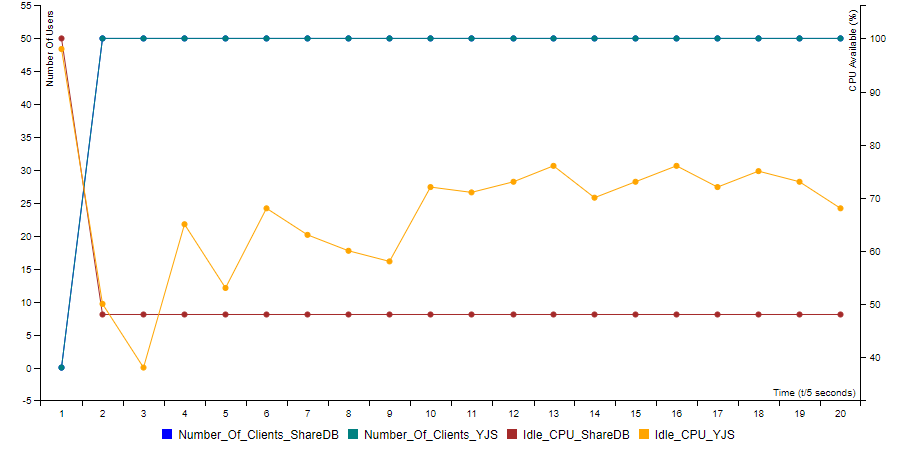
\includegraphics[scale=0.48]{scenario_a/users.png}

    \textbf{Scenario A}
    
    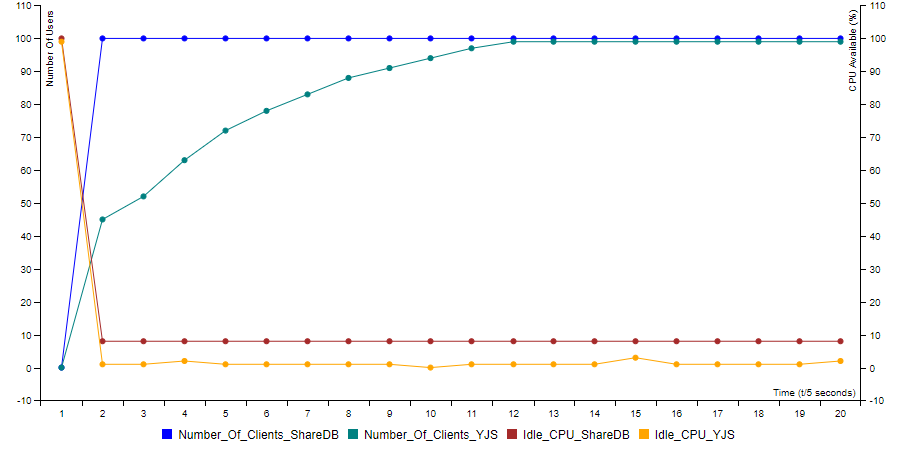
\includegraphics[scale=0.48]{scenario_b/users.png}
    
    \textbf{Scenario B}
    
    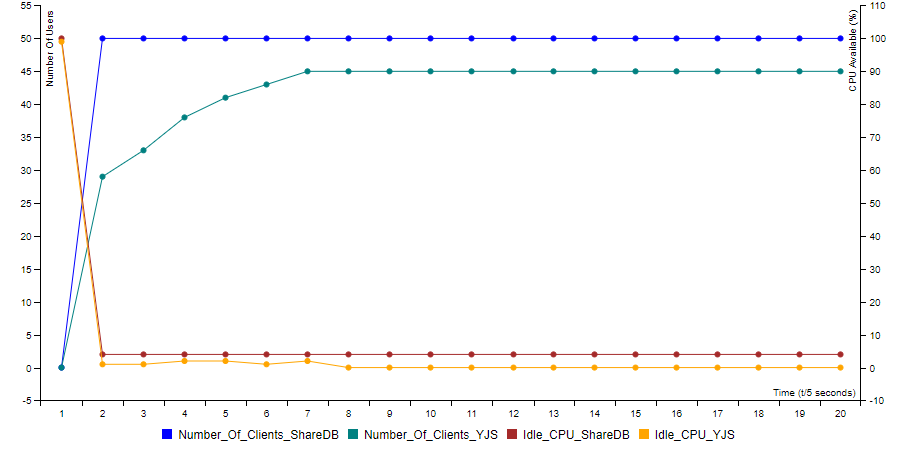
\includegraphics[scale=0.48]{scenario_c/users.png}
    
    \textbf{Scenario C}

  \end{center}

  \subsection{Document Size}
  The performance for conflict resolution can be seen using the change in document size (pace of character insertions).
  Interestingly when the CPU is not fully utilized (Scenario A) the performance for both ShareDB and YJS is the same.
  Though once we fully utilize the CPU (Scenario C), the performance of ShareDB is better by a large margin.
  \begin{center}
    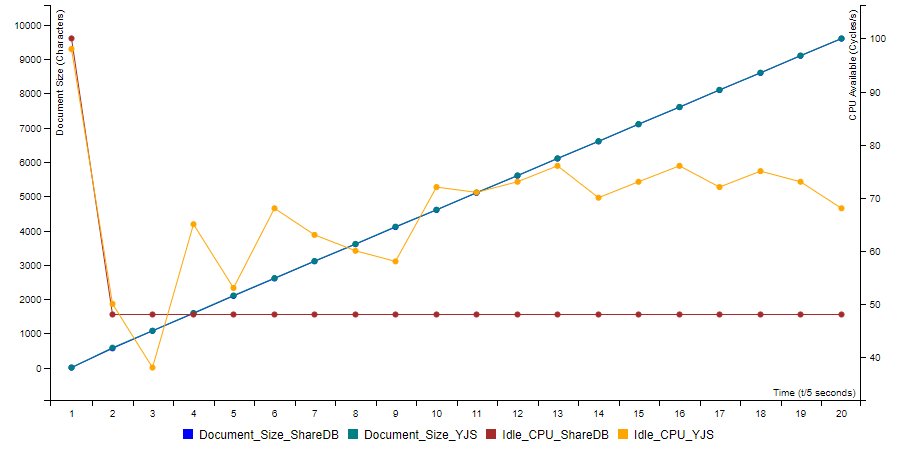
\includegraphics[scale=0.48]{scenario_a/document.png}

    \textbf{Scenario A}
    
    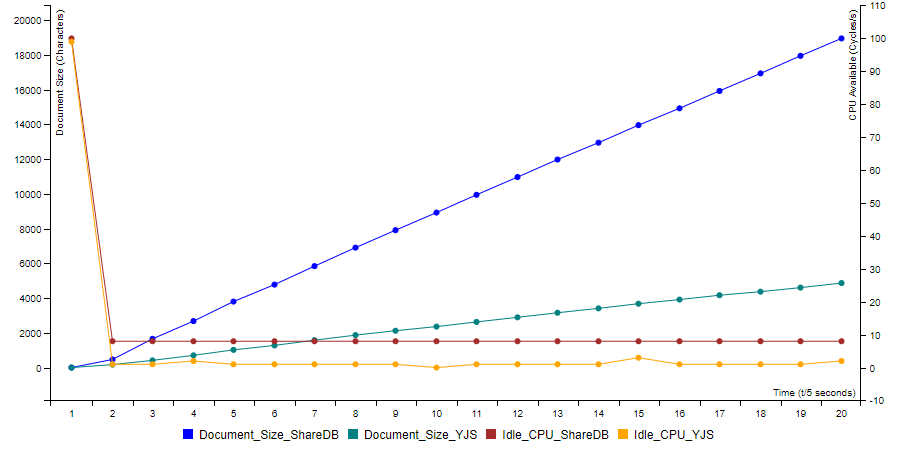
\includegraphics[scale=0.48]{scenario_b/document.png}
    
    \textbf{Scenario B}
    
    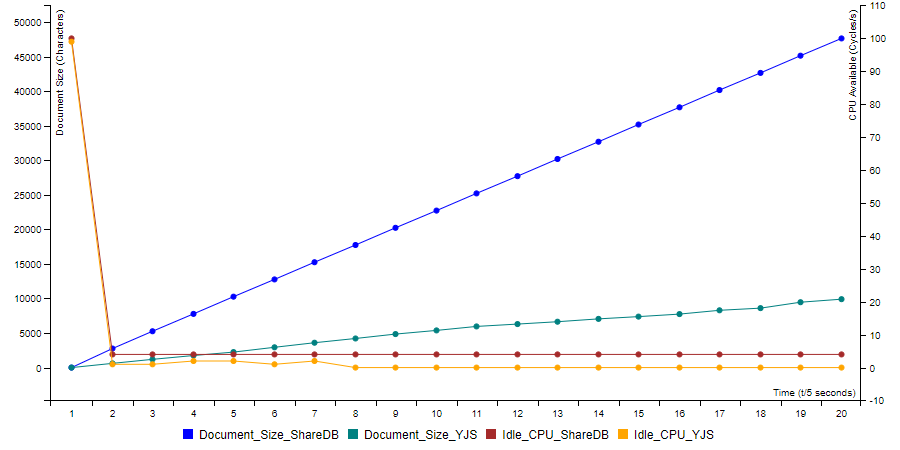
\includegraphics[scale=0.48]{scenario_c/document.png}
    
    \textbf{Scenario C}
  \end{center}

  Further looking at the below process information verifies that YJS has a higher per client CPU utilization. The top node process for both YJS and ShareDB is the server. The five node processes below in the list are the clients.
  The average CPU utilization per client for YJS is higher than that of ShareDB.
  
  \subsubsection{YJS}
  \begin{center}
    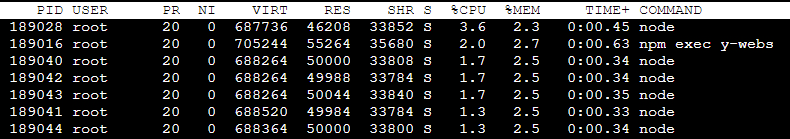
\includegraphics[scale=0.60]{yjs_processes.png}
  \end{center}

  \subsubsection{ShareDB}
  \begin{center}
    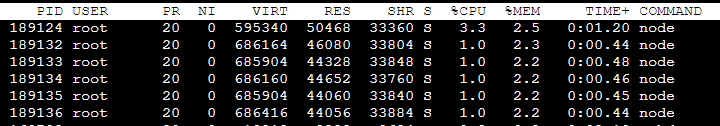
\includegraphics[scale=0.60]{sharedb_processes.PNG}
  \end{center}

  \subsection{Memory Utilization}
  Memory utilization is quite similar for both YJS and ShareDB, though a bit higher for YJS. This is also due to the fact that
  in CRDT approaches each client must maintain additional meta data for the document contents. Though generally this is not a 
  major issue as YJS is created for distributed utilization and hence the memory utilization is also distributed on several machines.
  \begin{center}
    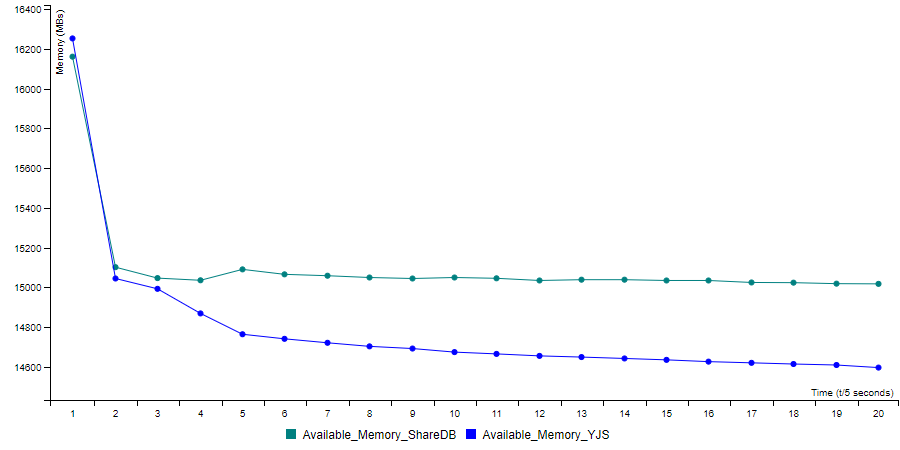
\includegraphics[scale=0.48]{scenario_a/memory.png}

    \textbf{Scenario A}
    
    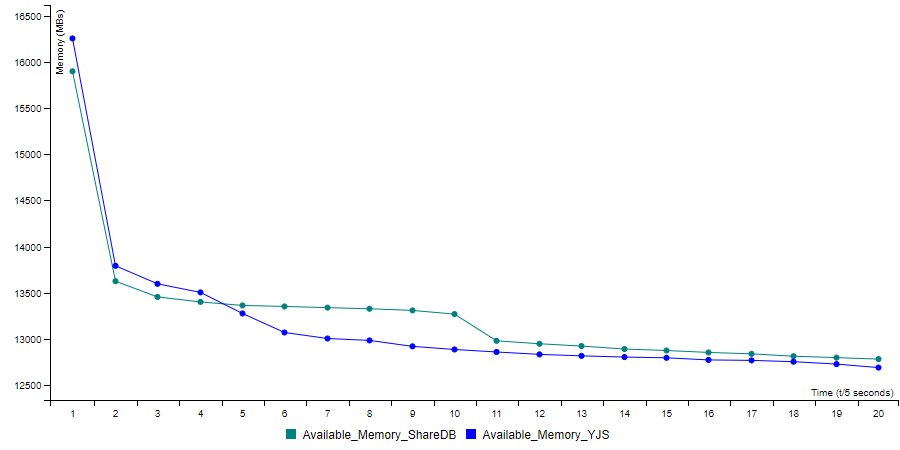
\includegraphics[scale=0.48]{scenario_b/memory.png}
    
    \textbf{Scenario B}
    
    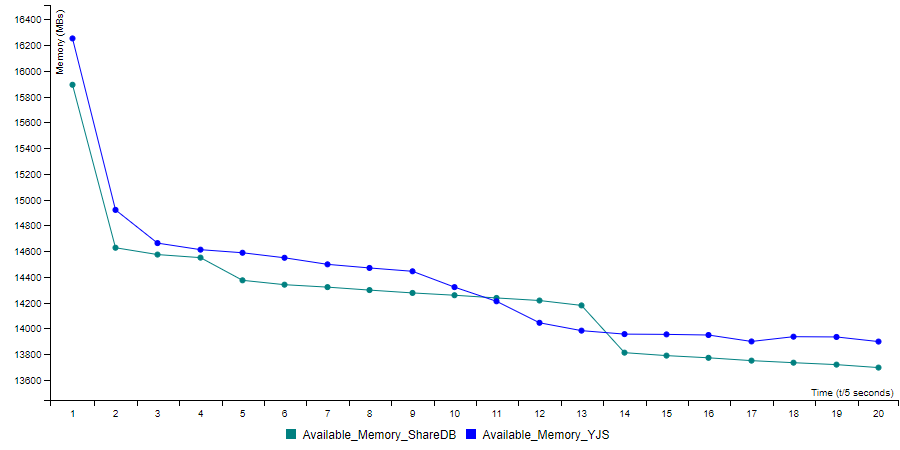
\includegraphics[scale=0.48]{scenario_c/memory.png}
    
    \textbf{Scenario C}

  \end{center}

  \subsection{Accuracy}
  Previously we have looked at the hardware resource utilization per client for both YJS and ShareDB. In such comparisons as noted ShareDB does
  perform slightly better than YJS. Now we zoom in to look at the accuracy of the actual text produced when inserting characters.
  This is so that we can ascertain the "quality" of the conflict resolution that each approach offers, rather than simply the "quantity".
  We define a accuracy metric based on a simpler version of our insertion algorithm as shown in the below equation

  \begin{equation} \label{simple_insertion_algorithm_character}
    Char(index, id) = alphabet[index\ mod\ 26]
  \end{equation}

  \begin{equation} \label{overall_accuracy_measure}
    Accuracy(text, clients) = 100 - ErrorRate(text, clients)
  \end{equation}

  \begin{equation} \label{overall_accuracy_measure}
    ErrorRate(text, clients) = (\sum Err(text[index], index, clients)) \div length(text)
  \end{equation}

  \begin{equation} \label{error_calculation}
    Err(c, i, n) = 
    \left\{
	    \begin{array}{ll}
        1 & \mbox{if } alphabet[ceil(((i\ mod\ n * 26) + 1) \div n)-1] \neq c \\
        0 & \mbox{otherwise }
	    \end{array}
    \right.
  \end{equation}

  The indices in equations above start from 0 and alphabet is the list of alphabet a to z, in ascending order.
  
  \subsubsection{YJS}
  yyxxwwvvuuttssrrqqppoonnmmllkkjjiihhggffeeddccbbaa \ zzyyxxwwvvuuttssrrqqppoonnmmllkkjjiihhggffeeddccbbaa \ zzyyxxwwvvuuttssrrqqppoonnmmllkkjjiihhggffeeddccbbaa \ zzyyxxwwvvuuttssrrqqppoonnmmllkkjjiihhggffeeddccbbaa \ zzyyxxwwvvuuttssrrqqppoonnmmllkkjjiihhggffeeddccbbaa \ zzyyxxwwvvuuttssrrqqppoonnmmllkkjjiihhggffeeddcc1bba0

  \subsubsection{ShareDB}
  yyxxwwvvuuttsrsrqpqopnomnlmkljkjihighfgfedecdbcab az yzxywxwvvutustrsqrpqopnonmmllkjkjiihghfgefdecdbcab az yzxywxvwuvtustrsqrpqopnomnlmkljkjihighgffeeddcbcab az zyyxxwwvvuuttssrrqqppoonnmmllkjkijihhggfefeddccbbaa \ zzyyxxwwvvututsrsqrqpopnomnlmkljkijhighfgefdecdbcab a zzyyxxwwvuvtustrsqrpqopnomnlmkljkijhighfgefdecdbc1ba0

  \section{Conclusion}
  The CRDT implementation in YJS has it's advantages when compared to traditional Operational Transformation based approaches, but it also has disadvantages when compared along some performance dimensions.
  Based on our testing and analysis, YJS should be the preferred library for NRT collaboration when intention preservation is of the utmost importance or when offline P2P collaboration needs to be supported.
  In other cases, operational transformation at this stage seems to perform well specially for a larger number of clients. Hence when client connectivity is of the utmost importance then ShareDB should be preferred.

\end{document}